\section{A Simple And Interpretable Deep Gated  Network}\label{sec:interpret}
\begin{figure}[h]
\begin{minipage}{0.4\columnwidth}
\centering
\resizebox{\columnwidth}{!}{
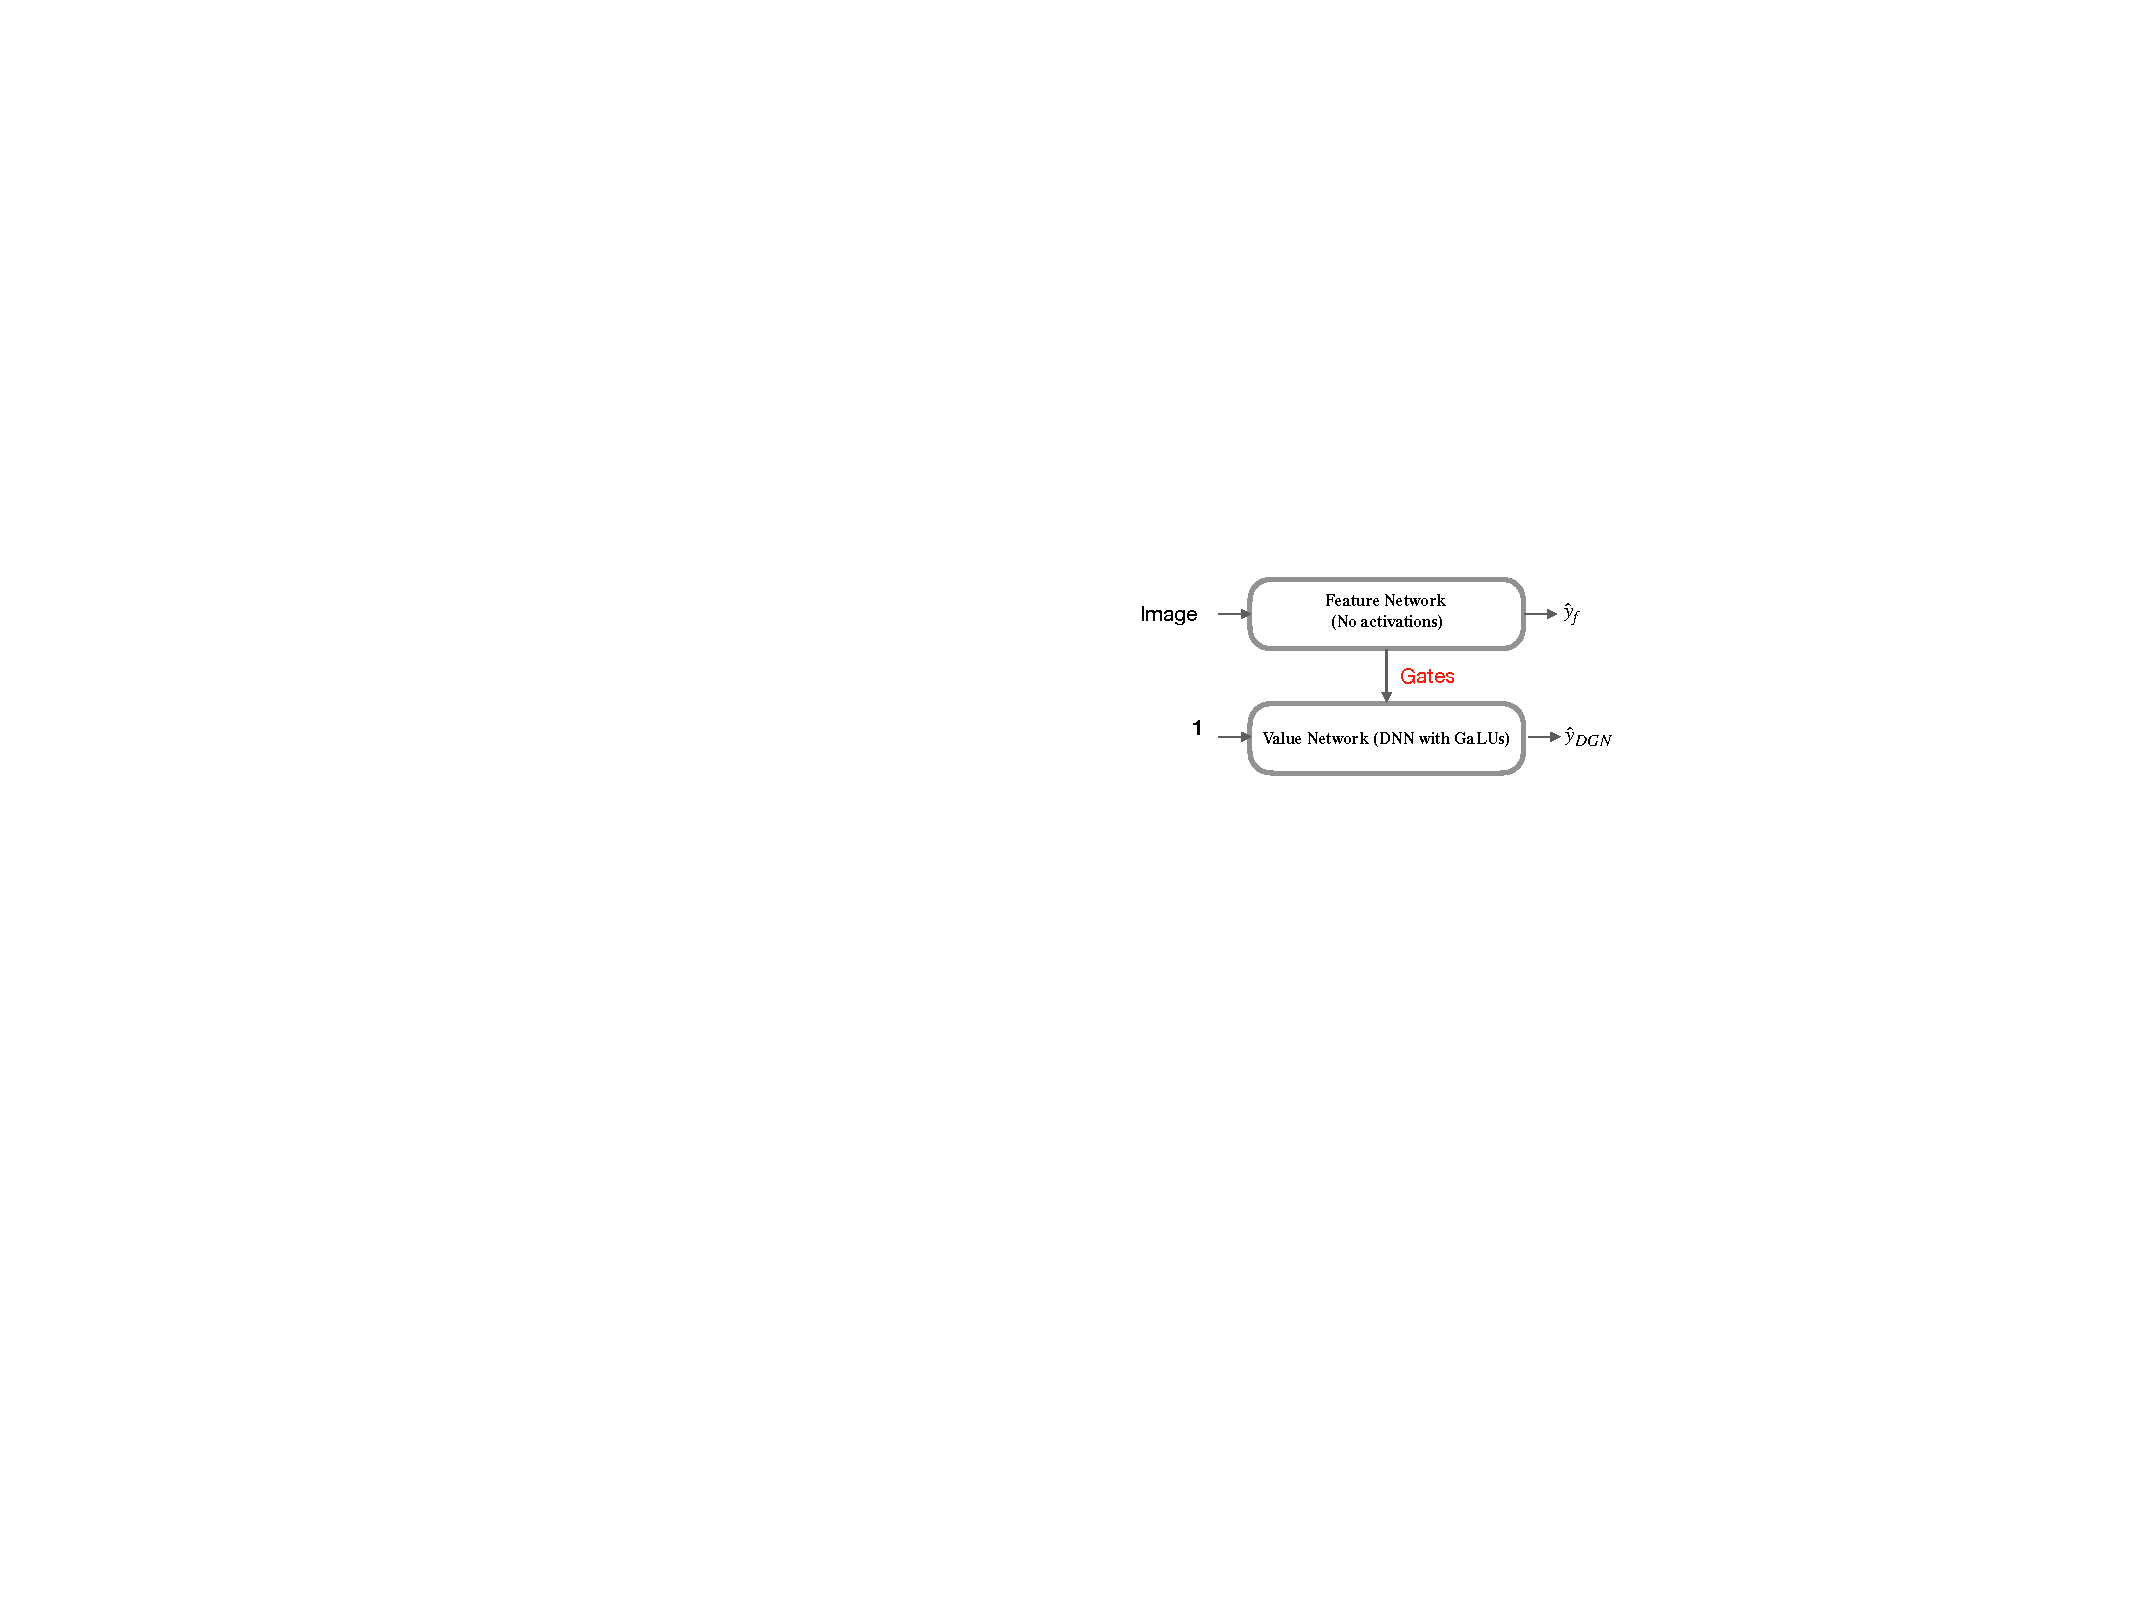
\includegraphics[scale=0.5]{figs/dgn-linear.pdf}
}
\end{minipage}
\begin{minipage}{0.4\columnwidth}
\begin{tabular}{rcc}
\toprule
&VGG19 & ResNet\\
Standard DNN& &\\
DGN-No-Act& & \\
\bottomrule
\end{tabular}
\end{minipage}
\end{figure}

\begin{comment}
\begin{wrapfigure}{r}{0.3\textwidth}
\resizebox{0.3\columnwidth}{!}{
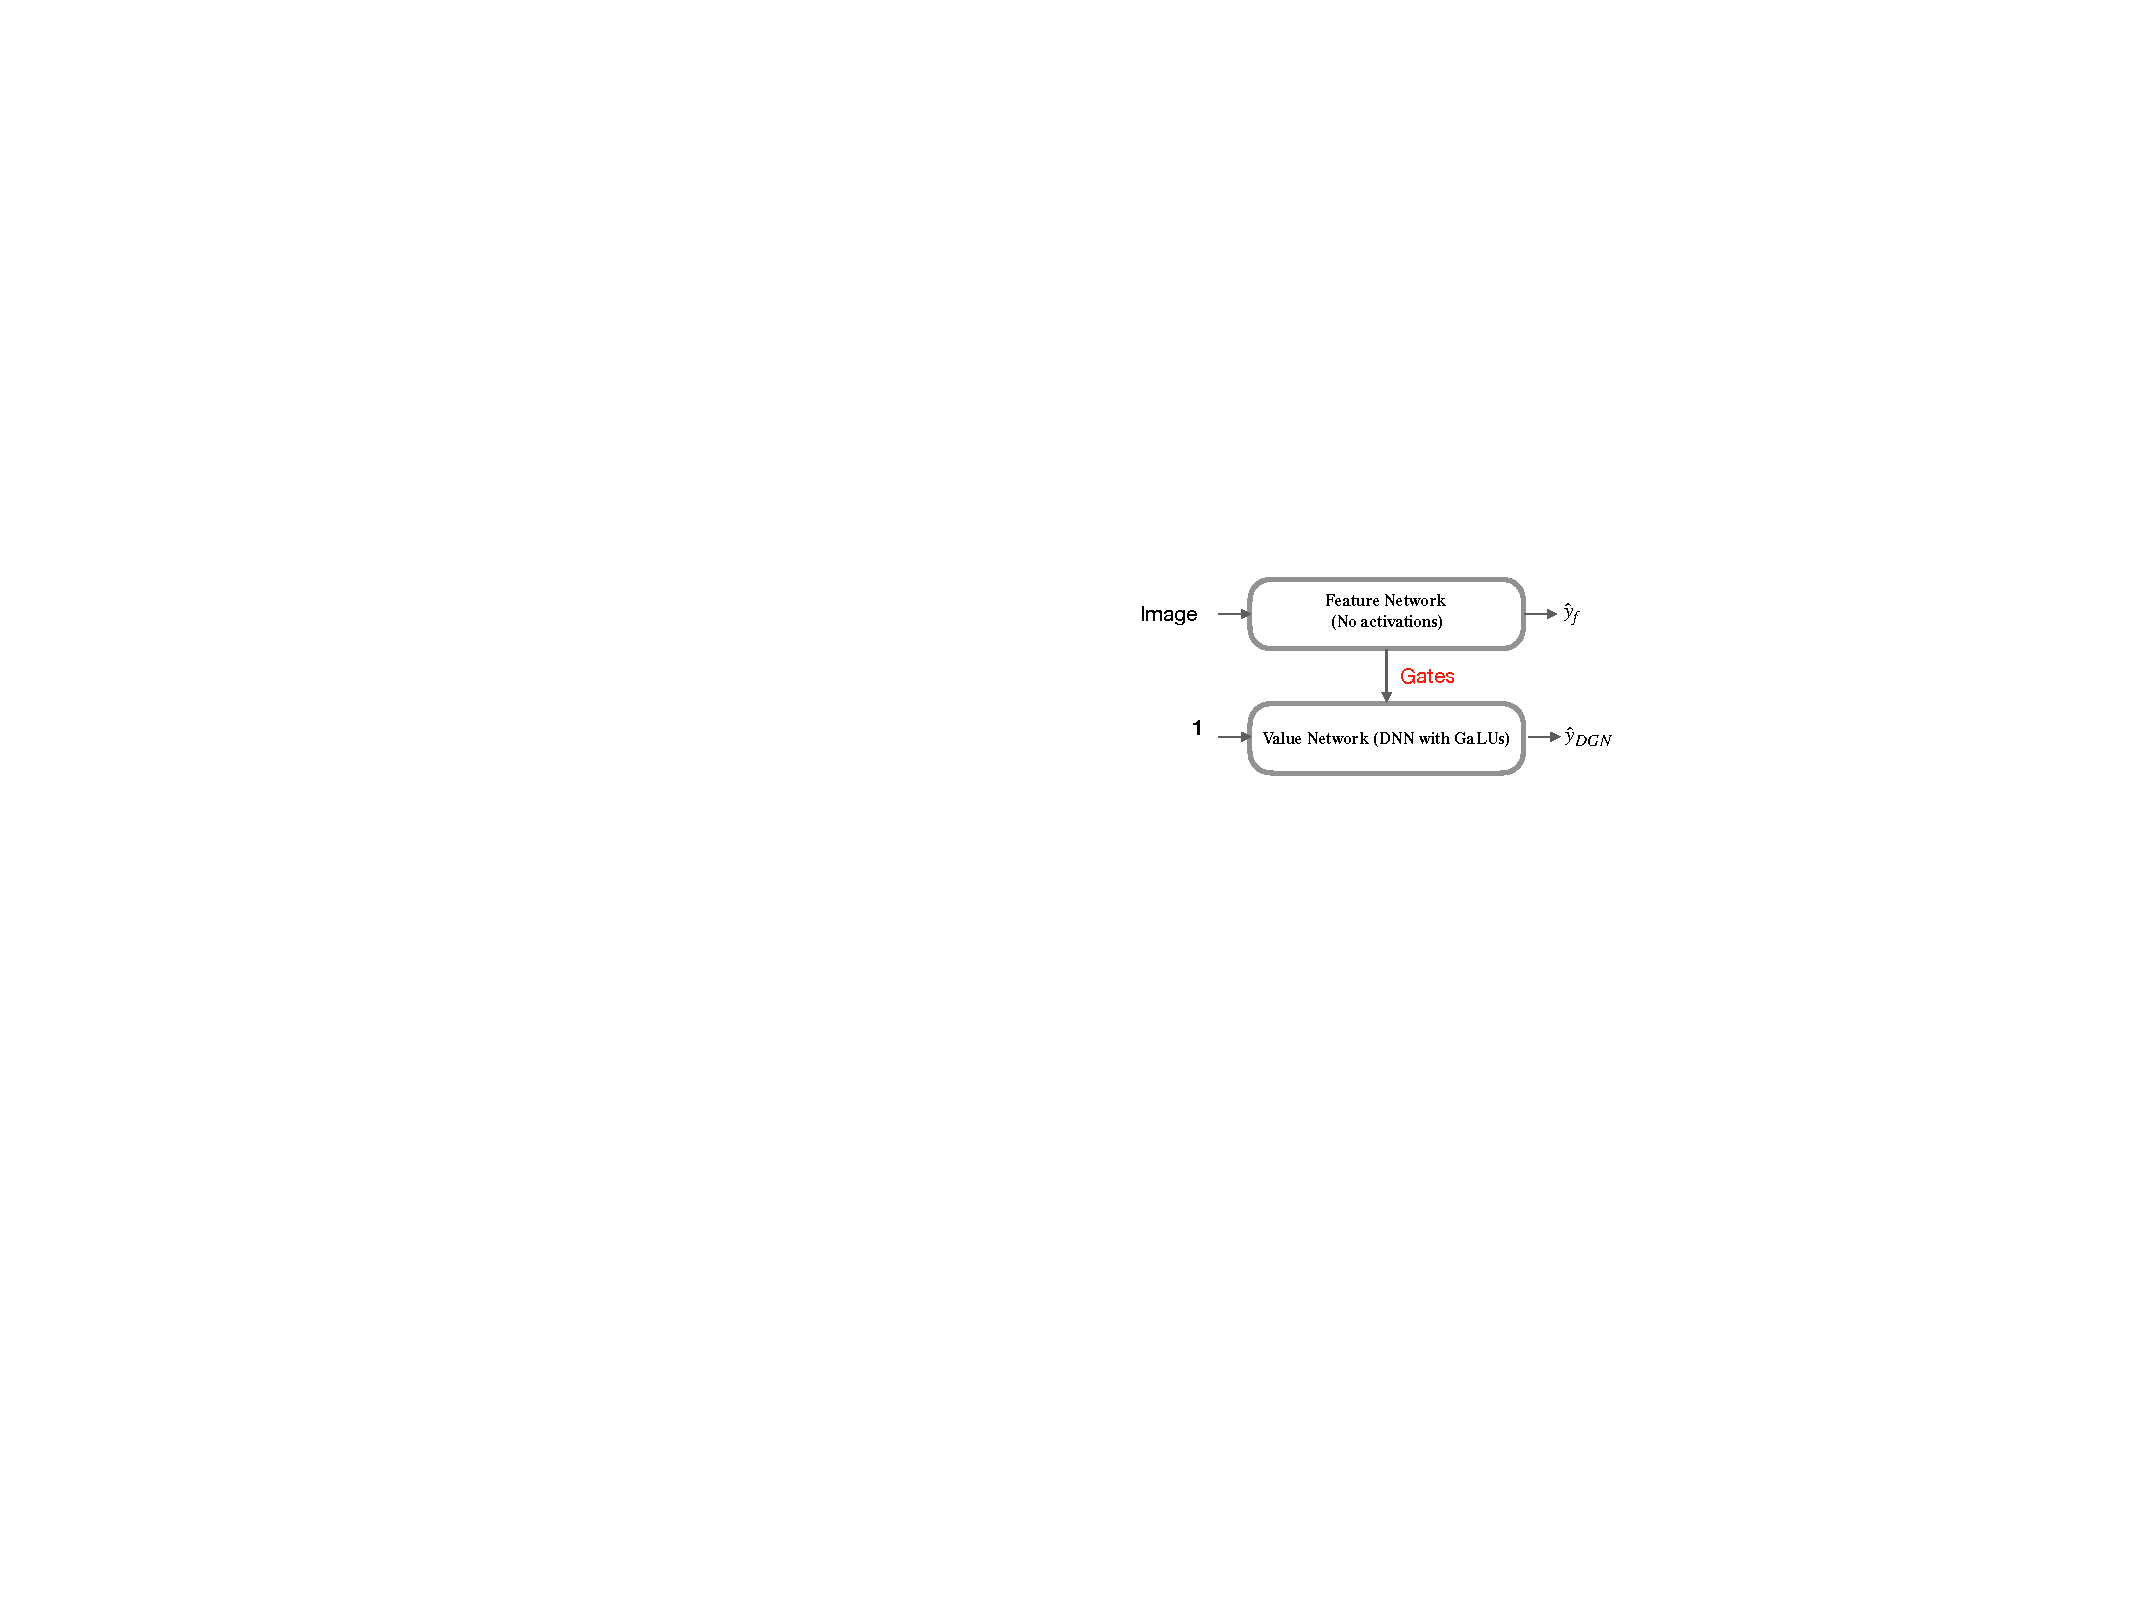
\includegraphics[scale=0.5]{figs/dgn-linear.pdf}
}
\end{wrapfigure}
\end{comment}
Till now we were interested in `what is learnt in a DNN with ReLUs'. We answered this question using the DGN setup.  We now ask the following question: `What happens if we remove activations (i.e., replace it with identity activations) from the feature network of a DGN?'-- let us call this the \emph{DGN-No-Act}. The motivation is that, once the activations are removed from the feature network, then feature generation will no longer be hidden, i.e., it will only be in terms of transformations such as matrix multiplication, pooling and scale/mean correction (in the case of batch norm), all of which have concrete `image processing'  interpretations. The gates in DGN-No-Act are derived (as usual) from the pre-activations of the identity activations in the feature network. The value network in the DGN-No-Act has the same functionality, i.e., it learns the NPV. We constructed two such `DGN-No-Act's based on standard architectures (VGG19 and an off-the-shelf ResNet), wherein, the standard architecture is used in feature network (without ReLU) and in the value network with ReLU replaced by GaLU. Both these DGN-No-Acts gave more than $90\%$ test accuracy on CIFAR-10.

%We answered this question using the DGN setup, where the DNN with ReLU which we want to study is the feature network, and we measured the performance by training the value network. 
%Based on the insights obtained from \Cref{th:main}, especially those on the roles of feature and value networks, and further experiments on how gate learning happens,